\documentclass[12pt,twoside]{article}
\usepackage[a4paper,width=150mm,headheight=110pt,top=25mm,bottom=25mm]{geometry}
\usepackage[utf8]{inputenc}
\usepackage{amsfonts}
\usepackage{amsmath}
\usepackage{amssymb}
\usepackage{pgfplots}

\title{MAT0206 - Prova 2}
\author{Matheus T. de Laurentys, 9793714}

\newcommand{\acc}{acumulação}
\newcommand{\defi}{definição}
\newcommand{\adh}{aderência}
\newcommand{\n}{não }
\newcommand{\ent}{então }
\newcommand{\Ent}{Então }
\newcommand{\eh}{é }
\newcommand{\seq}{sequência}
\newcommand{\num}{número}
\newcommand{\sao}{são }
\newcommand{\tambem}{também }
\newcommand{\cont}{contínua}
\newcommand{\contradicao}{contradição}
\newcommand{\vizin}{vizinhança }

\newcommand{\limi}[2]{$\displaystyle{\lim_{n \to +\infty}}(#1)=#2$}
\newcommand{\f}{\mkern-2mu f\mkern-3mu}
\newcommand{\R}{\mathbb{R}}
\newcommand{\N}{\mathbb{N}}

\begin{document}
	\maketitle
	
	\noindent\textbf{Provas Auxiliares:}\\
	
	$\mathbb{Q}\setminus\mathbb{Z}$ \eh denso em $\R$:
	
	[Por \contradicao] Seja $(a,b) \subset \R$ tal que $\nexists x \in \mathbb{Q}\setminus\mathbb{Z}$ tal que $x \in (a,b)$.
	Como $\mathbb{Q}$ \eh denso, \ent existe $x\in \mathbb{Z}$ tal que $x\in (a,b)$. Se existir outro inteiro no intervalo, \ent existe $y; |x-y| = 1$ no intervalo. \Ent $[x,y] \in (a,b)$ e isso implica que $\frac{b-a}{2} \in (a,b)$. Como $\frac{b-a}{2} \in \mathbb{Q}\setminus\mathbb{Z}$, tem-se \contradicao.
	
	Dessa forma, ha apenas um inteiro em $(a,b)$. Nesse caso, todavia, tem-se $(a,z)\cup (z,b) \subset (a,b)$ sem inteiros. Como $\mathbb{Q}$ \eh denso em $\R$, \ent $\exists q \in \mathbb{Q}$ tal que $q \in (a,x)$. Isso contradiz a suposição, pois $q \in (a,b)$. Tem-se \ent que $\nexists(a,b) \subset \R$ tal que $\nexists x \in \mathbb{Q}\setminus\mathbb{Z}$ tal que $x \in (a,b)$. Sendo assim, $\mathbb{Q}\setminus\mathbb{Z}$ \eh denso em $\R$.\\
	
		
	\noindent\textbf{Q.1:}
	
	$(x_n)_{n\in\mathbb{N}}, (y_n)_{n\in\mathbb{N}}$ \seq s de \num s reais.
	
	$A$ = limsup $x_n$ e $B$ = limsup $y_n$.
	
	\noindent\textbf{a)} lim inf $(-x_n) = - A$
	
	Como visto em aula, limsup $x_n$ \eh\ o maior limite de qualquer sub\seq\ convergente de $(x_n)_{n\in\N}$ e liminf $x_n$ o menor desses limites.
	
	Considere a \seq\ $(B, \ldots, A)$, de pontos que \sao limites de sub\seq s de $(x_n)_{n\in\mathbb{N}}$,  ordenada de maneira \n decrescente.
	
	Se $x\in\mathbb{R}$ \eh limite de sub\seq\ de $(x_n)$, \ent $-x$ \eh limite de \seq\ de $(-x_n)$. Se $x\in\mathbb{R}$ \eh limite de sub\seq\ de $(-x_n)$, \ent $-x$ \eh limite de \seq\ de $(x_n)$
	
	\noindent [Prova] Tome $(z_n)_{n\in\mathbb{N}}$ sub\seq\ de $(x_n)_{n\in\mathbb{N}}$ tal que \limi{z_n}{x}. 
	\Ent $(a_n)_{n\in\mathbb{N}}$, dada por $\forall i\in\mathbb{N}, a_i = -z_i$, \eh\ sub\seq\ de $(-x_n)_{n\in\mathbb{N}}$ tal que \limi{a_n}{-x}, pois $\forall \epsilon > 0, \exists a_i \in (a_n)_{n\in\mathbb{N}}$ tal que $|a_i - (-x)| < \epsilon$. Isso \eh\ verdadeiro pois $\forall \epsilon > 0, \exists z_i \in (z_n)_{n\in\mathbb{N}}$ tal que $|z_i -  x| < \epsilon$. Essa mesma prova \tambem mostra que se $x\in\mathbb{R}$ \eh\ limite de sub\seq\ de $(-x_n)$, \ent $-x$ \eh\ limite de \seq\ de $(x_n)$
	
	Sendo assim, $(-B,\ldots,-A)$ \eh a \seq\ de pontos que \sao limites de sub\seq s de $(-x_n)_{n\in\mathbb{N}}$. Toma-se \ent a \seq\ ordenada $(-A,\ldots,-B)$ de tais limites. Como liminf \eh o menor desses limites, \ent \hbox{liminf$(-x_n) = -A$}.\\
	
	
	\noindent\textbf{b)} Seja \limi{x_n}{x_0}. Mostre limsup $(x_n - y_n) \ge x_0 - B$.
	
	Como \limi{x_n}{x_0}, \ent a \seq\ \eh convergente e, assim, tem apenas um ponto de limite, $x_0$. Logo, limsup $(x_n) = x_0$. Pode-se, \ent, re-escrever limsup $(x_n - y_n) \ge x_0 - B$ como limsup $(x_n - y_n) \ge \text{limsup}(x_n) - \text{limsup}(y_n) = A - B$.
	
	[Por \contradicao] Suponha que limsup $(x_n - y_n) < A - B$. Tome $\epsilon = A - B -$ limsup$(x_n - y_n)$. $\epsilon > 0$ 
	
	Como existem sub\seq s de $(x_n)_{n\in\N}$ e $(y_n)_{n\in\N}$ tais que seus limites sejam $\text{limsup}(x_n)$ e $\text{limsup}(y_n)$, \ent $\forall N \in \N$, $\exists n \ge \N$, $|x_n - A| < \frac{\epsilon}{4}$ e $|y_n - B| < \frac{\epsilon}{4}$. Sendo assim, $A - \frac{\epsilon}{4} < x'_n < A + \frac{\epsilon}{4}$ e $B - \frac{\epsilon}{4} < y'_n < B + \frac{\epsilon}{4}$.
	
	Temos \ent que
	
	$$
	A - B - \frac{\epsilon}{2} = A - \frac{\epsilon}{4} - (B - \frac{\epsilon}{4}) < x'_n - y'_n < A + \epsilon - B - \epsilon = A - B
	$$
	
	Como $\epsilon$
	
	a\\
	
	
	\noindent\textbf{Q.2:}\\
	
	
	\noindent\textbf{a)} $X_\alpha := \{m+n.\alpha; m\in\mathbb{Z} \text{ e }n \in\mathbb{Z}\}$ e $\alpha$ irracional.
	Sejam $\f :\R\rightarrow\R$ e $g: \R\rightarrow\R$ \cont s.
	$\forall x \in X, \f (x) = g(x)$. Prove $\f = g$.
	
	[Por \contradicao] $\exists x_0 \in \R; f(x_0) \neq g(x_0)$.
	
	Seja $\epsilon < f(x_0) - g(x_0), \epsilon \neq 0$. Considere que $\epsilon > 0$, sem perda de generalidade. Como $\f - g$ tambem \eh \cont\, \ent $\exists \delta > 0$ tal que $\forall x \in (x_0 - \delta, x_0 + \delta)$, $\f (x) - g(x) \in (\f (x_0) -g(x_0) - \epsilon, \f (x_0) -g(x_0) + \epsilon))$. Sendo assim, existe uma \vizin $V = (\f (x_0) -g(x_0) - \epsilon, \f (x_0) -g(x_0) + \epsilon)$ de $x_0$ tal que $\forall x \in V, |f(x) - g(x)| \ge \f (x_0) -g(x_0) - \epsilon > 0$. A segunda desigualdade vale pela escolha de $\epsilon$.
	
	Porem, como os irracionais \sao densos em $\R$, \ent $\exists \alpha \in V, \alpha$ \eh irracional. Isso contradiz o fato de $\forall x$ irracional, $f(x) = g(x)$. Logo, $\nexists x_0 \in \R; f(x_0) \neq g(x_0)$. Sendo assim $\forall x \in \R, f(x) = g(x)$ e isso mostra que $f = g$.\\
	
	
	\noindent\textbf{b)} a) \eh verdadeiro caso $\alpha$ seja racional?\\
	
	Sim, esse caso tambem \eh verdadeiro e, na verdade, a prova \eh a mesma.
	
	Segue, de qualquer forma, a prova desse caso.
	
	[Por \contradicao] $\exists x_0 \in \R; f(x_0) \neq g(x_0)$.
	
	Seja $\epsilon < f(x_0) - g(x_0), \epsilon \neq 0$. Considere que $\epsilon > 0$, sem perda de generalidade. Como $\f - g$ tambem \eh \cont\, \ent $\exists \delta > 0$ tal que $\forall x \in (x_0 - \delta, x_0 + \delta)$, $\f (x) - g(x) \in (\f (x_0) -g(x_0) - \epsilon, \f (x_0) -g(x_0) + \epsilon))$. Sendo assim, existe uma \vizin $V = (\f (x_0) -g(x_0) - \epsilon, \f (x_0) -g(x_0) + \epsilon)$ de $x_0$ tal que $\forall x \in V, |f(x) - g(x)| \ge \f (x_0) -g(x_0) - \epsilon > 0$. A segunda desigualdade vale pela escolha de $\epsilon$.
	
	Porem, como os racionais \sao densos em $\R$, \ent $\exists \alpha \in V, \alpha$ \eh racional. Isso contradiz o fato de $\forall x$ racional, $f(x) = g(x)$. Logo, $\nexists x_0 \in \R; f(x_0) \neq g(x_0)$. Sendo assim $\forall x \in \R, f(x) = g(x)$ e isso mostra que $f = g$.\\
	
	
	\noindent\textbf{c)} $\f :\R\rightarrow\R$ \cont. Existe $g: \R\rightarrow\R$ des\cont\ em todos os pontos com $\forall x \in X, \f (x) = g(x)$ e $\alpha$ irracional?\\
	
	Antes, provar que $\mathbb{Q}\setminus\mathbb{Z} \subset \R \setminus X_\alpha$:
	
	[Por \contradicao] Suponha $q \in \mathbb{Q}\setminus\mathbb{Z}$ e $q \notin \R \setminus X_\alpha$.
	
	Como $q \in \mathbb{Q}, q \in \R$. Sendo assim, $q \in X_\alpha$. Isso significa que $q = \frac{a}{b} = m + n\alpha$, sendo $a,n,m \in \mathbb{Z}, b\in\N, b\neq 1$. Se esse fosse o caso, $a = b.m + b.n.\alpha \rightarrow (a - b.m) = b.n.\alpha$. Como $(a - b.m) \in \mathbb{Z}, b.n.\alpha\in \mathbb{Z}$. Como $\alpha$ irracional, $\nexists z\in \mathbb{Z}$ tal que $z.\alpha \in Z$, mostrando que $b.n.\alpha\notin \mathbb{Z}$. Sendo assim, $q \notin X_\alpha$, e, consequentemente, $q \in \R \setminus X_\alpha$. Isso mostra que $\mathbb{Q}\setminus\mathbb{Z} \subset \R \setminus X_\alpha$.\\
	
	Para a questão. Sim, existe tal $g$. Tome $g$ dada por:
	
	$
	\begin{cases}
		f(x), &\text{se } x \in X_\alpha\\
		f(x) + 10, &c.c.\text{ Note que isso inclui } \mathbb{Q}\setminus\mathbb{Z}
	\end{cases}
	$
	
	[Por \contradicao] Seja $x_0 \in \R$ tal que $g$ \eh \cont\ em $x_0$.
	
	Como $g$ \cont em $x_0$, \ent $\forall \epsilon > 0, \exists \delta > 0$ tal que $\forall x \in (x_0 - \delta, x_0 + \delta)$, \hbox{$g(x) \in (g(x_0) - \epsilon, g(x_0) + \epsilon)$}. Seja, \ent, algum $\epsilon > 0$ e $\epsilon < 10$. Como $C = \mathbb{Q}\setminus\mathbb{Z}$ denso em $\R$, qualquer que seja $\delta > 0$, $\exists q \in C$ tal que $q \in (x_0 - \delta, x_0 + \delta)$. Como $g(q) = g(x_0) + 10, g(q)\notin (g(x_0) + \epsilon, g(x_0) + \epsilon)$. Isso contradiz o fato de $g$ ser \cont\ em $x_0$. Sendo assim, $g$ \eh des\cont\ em todos os pontos.\\
	
	
	\noindent\textbf{Q.3} Sejam $A$ e $B$ conjuntos compactos tais que $A \neq \emptyset, B \neq \emptyset, A \subset \R, B \subset \R$. $d(A,B) = inf\{|a-b|; a\in A \text{ e } b\in B\}$\\
	
	
	\noindent\textbf{a)} $(A \cap B = \emptyset) \Rightarrow d(A,B)>0$
	
	[Por \contradicao]
	Sejam $a \in A, b\in B$ tais que $|a-b| = 0$.
	
	Tome $\epsilon > 0$. Como $|a-b| = 0$, $b\in (a-\epsilon, a+\epsilon)$. Sendo assim, $a \in \partial B$. Como B \eh fechado, tem-se \contradicao pois conjuntos fechados contem sua fronteira (visto em L4 E10c). Sendo assim, $\nexists a \in A, b \in B$ tais que $|a-b| = 0$. Assim, $|a-b| \neq 0$.
	
	Como $|a-b| \ge 0, \forall a, b \in \R$, \ent $d(A,B)>0$.\\


	\noindent\textbf{b)}$(A \cap B = \emptyset) \Rightarrow \exists a\in A, b \in B; d(A,B)=|a-b|$
	
	Tem-se que $\forall a\in A, b\in B$, $d(A,B) \leq |a-b|$ imediatamente pois $\forall a\in A, b\in B$, $|a-b| \in {|a-b|; a\in A, b\in B}$ e $\forall x \in X$. inf$X \leq x$ por \defi.\\
	
	[Por \contradicao] Seja, $\forall a\in A, b\in B$, $D = d(A,B) < |a-b|$.
	
	Como $D$ \eh infimo, \ent existe uma \seq\ de ${|a-b|; a\in A, b\in B}$ cujo limite \eh $D$. Seja $(x_n)_{n\in\N}$ uma tal \seq\. Tome $\epsilon>0,\exists N \in \N, \forall n \ge N, |x_n - D| < \epsilon$. Por \defi $x_n = |a-b|, a\in A, b\in B$. Porem, se fixado $\epsilon = d(A,B) - |a-b|$, \ent existem $a\in A, b\in B$ com $|(a-b)-D| < d(A,B) - |a-b|$, 

	\noindent\textbf{c)} De exemplos de $A,B \subset \R$ fechados tais que $A \neq \emptyset, B \neq \emptyset, A\cap B = \emptyset, d(A,B) = 0$.

	Tome $A = \mathbb{N}$ e $B = \{n + \frac{1}{n}; n \in \N\}$. Ambos tem apenas pontos isolados, e por isso, \sao fechados. Assim, $inf\{|n - n + \frac{1}{n}|\} = inf\{|\frac{1}{n}|\} = 0$.
	
	Mantendo B, pode-se tomar $A' = A \setminus \{n_1, n_2, \ldots, n_k; n_i \in \N\ \text{quaisquers}\}$.
	
	Mantendo A, pode-se tomar $B' = \{n + \f . \frac{1}{n}\; n \in \N, \f \text{ limitada}\}$\\
	
	
	\noindent\textbf{EXTRA}\\
	
	
	\noindent\textbf{a)} $\f\;$ tem a propriedade (U) $\iff$ \hbox{$\forall (x_n)_{n\in\N}$ em X com \limi{x_n}{x_0} tem-se limsup $\f (x_n) \leq \f (x_0)$}.
	
	($\Rightarrow$)
	
	[Por \contradicao] Seja $(x_n)_{n\in\N}$ em X com \limi{x_n}{x_0}, mas \hbox{limsup $f(x_n) > f(x_0)$}.
	
	Seja $(y_n)_{n\in\N}$ sub\seq\ de $(x_n)_{n\in\N}$ tal que $L =$ lim$f(y_n) > f(x_0)$. Seja $\alpha =$ $\frac{L - f(x_0)}{2}$. Tome $0 < \epsilon < \alpha$. Como $f$ tem propriedade U, $\exists \delta > 0$ tal que $\forall x \in (x_0 - \delta, x_0 + \delta), f(x) \in (f(x_0) - \epsilon, f(x_0) + \epsilon)$. Porem, pela escolha de $\epsilon$, tem-se uma vizinhança $V=(x_0 - \delta, x_0 + \delta)$ de $x_0$ tal que $\nexists x \in V, f(x) \in (L - \alpha, L + \alpha)$, contradizendo o fato de $L$ ser limite. Sendo assim $\nexists (x_n)_{n\in\N}$ em X com \limi{x_n}{x_0}, mas \hbox{limsup $f(x_n) > f(x_0)$}. Logo, $\forall (x_n)_{n\in\N}$ em X com \limi{x_n}{x_0}, \hbox{limsup $f(x_n) \leq f(x_0)$} \\
	
	
	($\Leftarrow$)
	
	[Por \contradicao] Seja $\epsilon > 0$ de forma que $\nexists \delta > 0$ tal que \hbox{$\forall x \in (x_0 - \delta, x_0 + \delta)\cap X, f(x) < f(x_0) + \epsilon$}.
	
	Tome alguma \seq\ $(x_n)_{n\in\N}$ em X com \limi{x_n}{x_0}. Tome, \ent, $(y_n)_{n\in\N}$ sub\seq\ de $(x_n)_{n\in\N}$ tal que $L =$ lim$f(y_n) \leq f(x_0)$. Porem, como essa sub\seq\ converge para $L$, \ent $\exists N \in \N$ tal que $\forall n \ge N, |f(x_n) - L| < \epsilon$. Isso implica que $L - \epsilon < f(x_n) < L + \epsilon$. Porem, como $L \leq f(x_0)$, entao $f(x_n) \leq f(x_0) + \epsilon$. Isso contradiz a escolha de tal $\epsilon$. Por fim, isso mostra que $\forall \epsilon > 0 \exists \delta > 0; \forall x \in (x_0 - \delta, x_0 + \delta)\cap X, f(x) < f(x_0) + \epsilon$).\\
	
	
	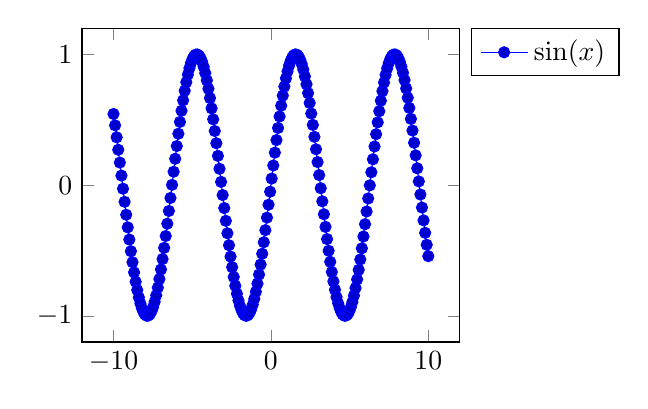
\begin{tikzpicture}
		\begin{axis}[domain=-10:10,legend pos=outer north east, samples=200, scale=0.7]
			\addplot {sin(deg(x))}; 
			\legend{$\sin(x)$}
		\end{axis}
	\end{tikzpicture}

	Nota: Poderia ser qualquer $f$ \cont em $x_0 = 0$.\\


	\textbf{b)} Note que se $f$ limitada superiormente, \ent ela assume valor máximo em X, pois ela \eh definida em X.
	
	Tome $x_0 = supX$ e $\epsilon>0$. Pela \defi, existe vizinhança de $x_0$ com $f$ limitada. Tomando $x_i < x_0$ nessa vizinhança, tem-se outra vizinhança limitada.
	
	Pode-se combrir os conjunto X com tais vizinhança. Porem, como visto em aula, toda familia de abertos cobrindo um compacto tem uma subfamilia finita que tambem o cobre. Tal familia mostra que $f$ \eh limitada superiormente pois sejam $x,y \in (a,b), f(x) < f(y) + \epsilon_1, f(y) < f(x) + \epsilon_2$.
\end{document}













